\subsection{Tiempo de ejecución}

En el punto de vista teórico, la fuerza bruta enumera trayectorias
y muestra un costo temporal correspondiente a $\binom{N+M-2}{N-1}$ 
en el peor caso \cite{algorithms_erickson}.
Por otro lado, la programación dinámica evalua cada celda considerando
las vidas disponibles, acotando su tiempo a $O(NMV)$, mientras que greedy
toma una única decisión local por paso en $O(N+M)$.

Los resultados observados en la \Cref{fig:tiempo} confirman este comportamiento.
En las grillas más pequeñas ($4\times4$), los tres paradigmas resuelven
cada instancia en fracciones de milisegundo; en este rango inicial, 
programación dinámica se ubica ligeramente por encima de los otros algoritmos
debido al costo fijo de inicializar su tabla de estados.
Al avanzar hacia el límite $N + M \le 32$,
fuerza bruta experimenta una explosión combinatoria que dispara su tiempo, 
punto en el cual se detiene su ejecución. A partir de allí, la curva de programación
dinamica describe una recta con pendiente constante, demostrando un escalamiento
lineal hasta las grillas de mayor tamaño. Greedy, 
en cambio, conserva la curva más baja.


\begin{figure}[H]
\centering
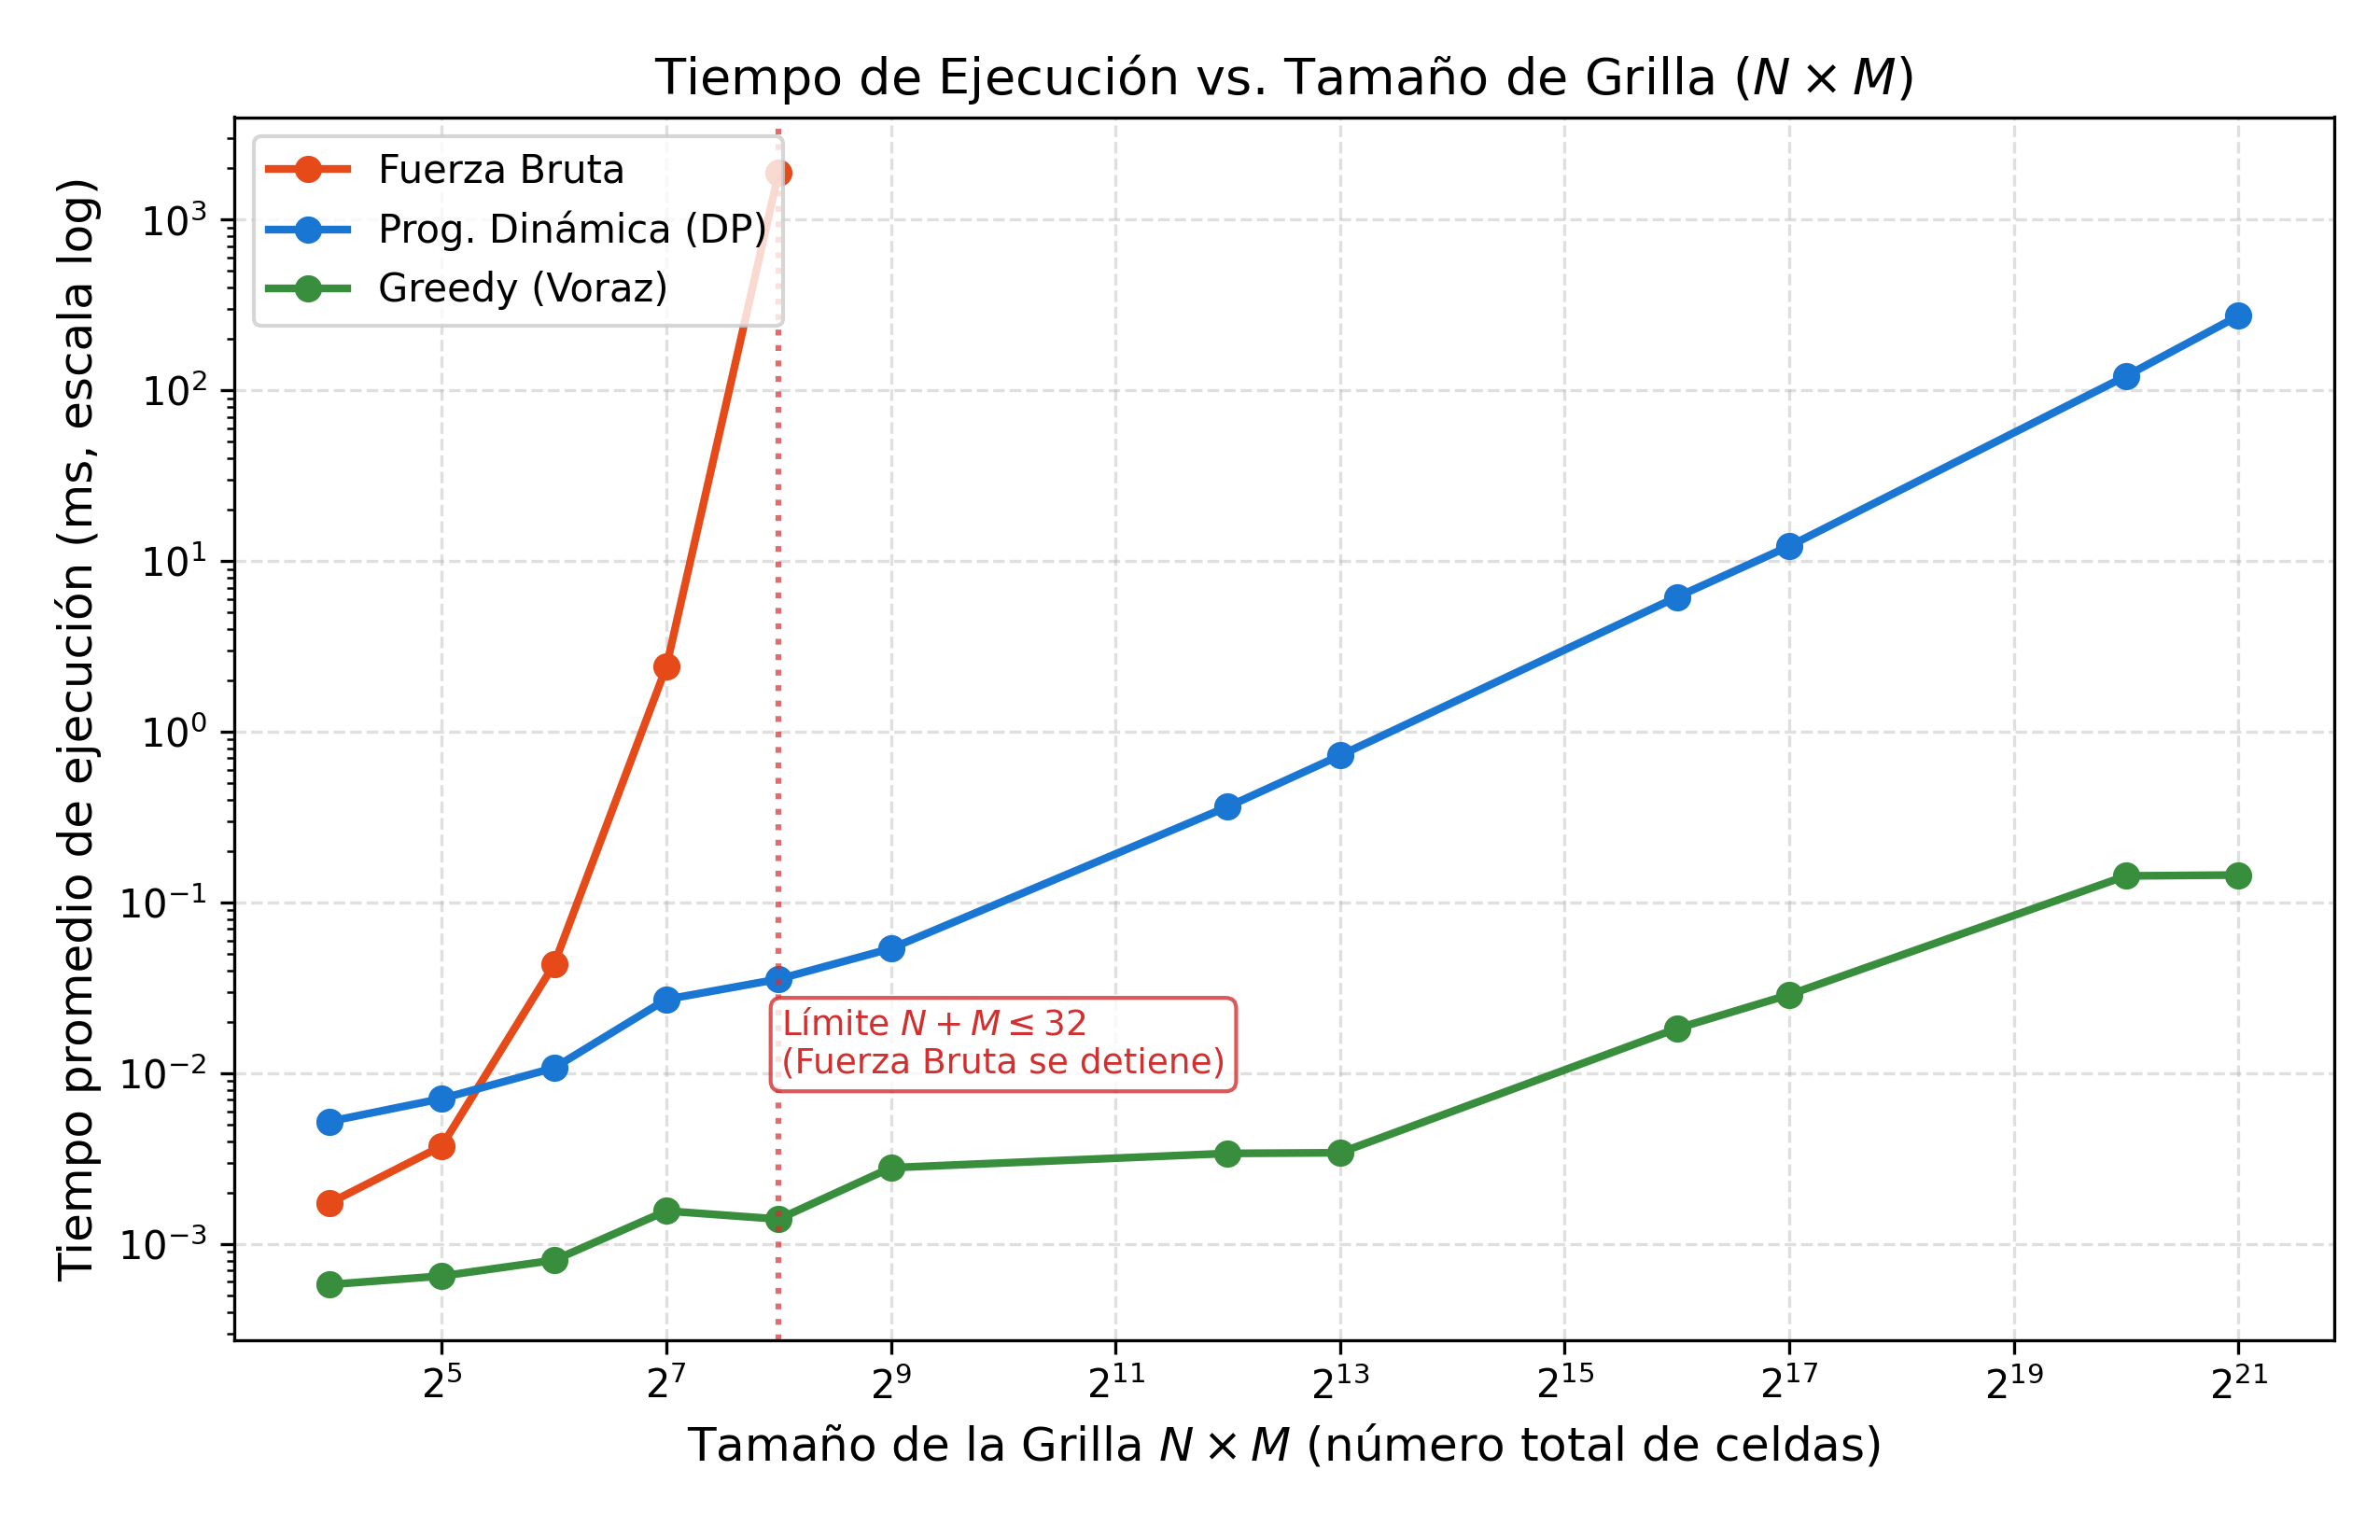
\includegraphics[width=0.83\linewidth]{../code/grid_pathfinding/data/plots/01_tiempo_vs_tamano.png}
\caption{Tiempo promedio de ejecución en función del número de celdas. La fuerza bruta se ejecuta únicamente hasta el límite $N+M=32$.}
\label{fig:tiempo}
\end{figure}




En la Figura~\ref{fig:tiempo-tipo} muestra cómo la presencia de obstáculos
modifica el comportamiento de cada algoritmo. 
En grillas \textit{libres} y con \textit{minas},
la fuerza bruta alcanza sus maximos de ejecución porque
todas las trayectorias siguen siendo validas hasta el destino. 
A diferencia en terrenos con \textit{murallas} y \textit{mixtos}, 
la poda temprana al chocar con celdas intransitables modera 
visiblemente el extremo superior de su curva.
Greedy de forma similar presenta ligeras irregularidades en su 
escalada pronunciada en grillas con murallas cuando queda atrapado y aborta 
de forma anticipada. Por el contrario, programación dinámica nos muestra curvas 
prácticamente idénticas en los cuatro paneles, confirmando que su tiempo de
ejecución es insensible a la distribución de los obstáculos al recorrer 
el espacio de estados.

\begin{figure}[H]
\centering
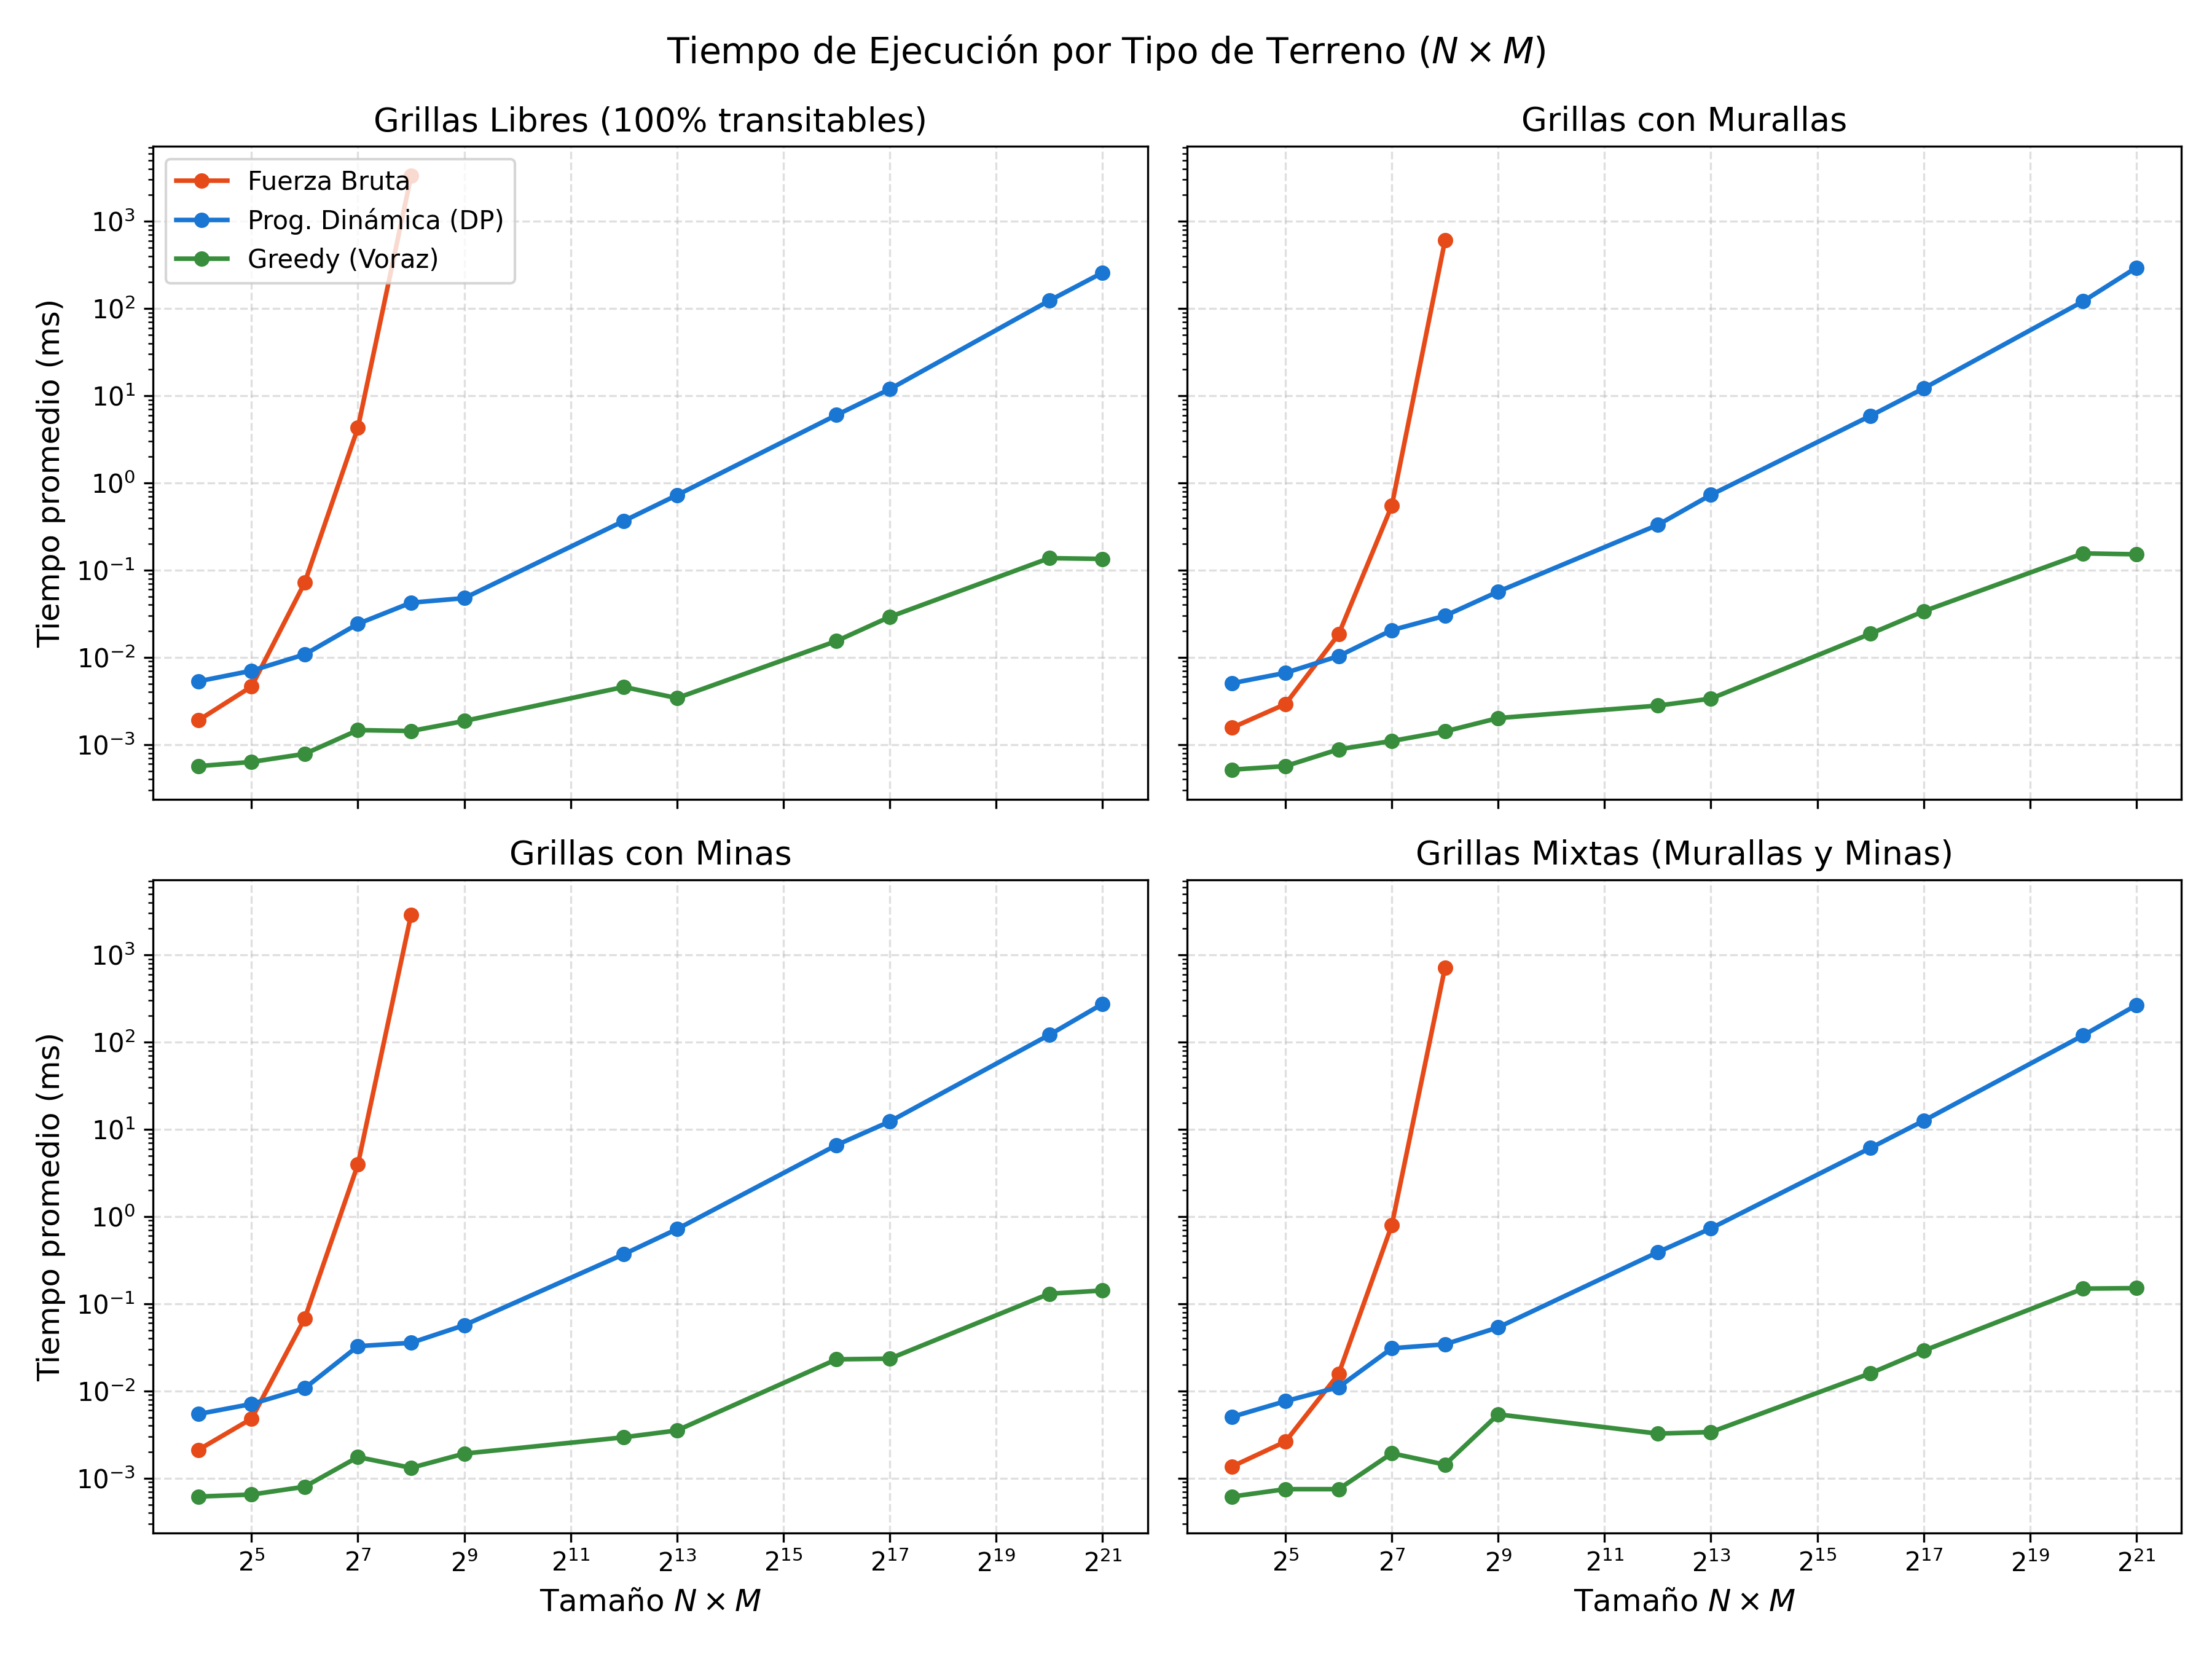
\includegraphics[width=0.83\linewidth]{../code/grid_pathfinding/data/plots/01b_tiempo_vs_tamano_por_tipo.png}
\caption{Tiempo promedio de ejecución por tamaño y tipo de grilla.}
\label{fig:tiempo-tipo}
\end{figure}

\subsection{Consumo de memoria}

La Figura~\ref{fig:memoria} se observa que la fuerza bruta 
y greedy requieren memoria proporcional a la longitud del camino, 
$O(N+M)$, programación dinámica escala como $O(NMV)$ para almacenar los 
puntajes óptimos parciales y la información necesaria
para reconstruir la trayectoria. Esta diferencia se manifiesta en 
las pendientes de las curvas: la memoria de programación dinámica crece 
de forma lineal, pasando desde el orden de unos
pocos kb en grillas pequeñas hasta alcanzar el orden de cientos
de mb en las instancias de $2^{20}$ celdas.
Por su parte, tanto la fuerza bruta como greedy 
mantienen un consumo de memoria reducido, escalando linealmente con la 
longitud de la trayectoria $O(N + M)$.

\begin{figure}[H]
\centering
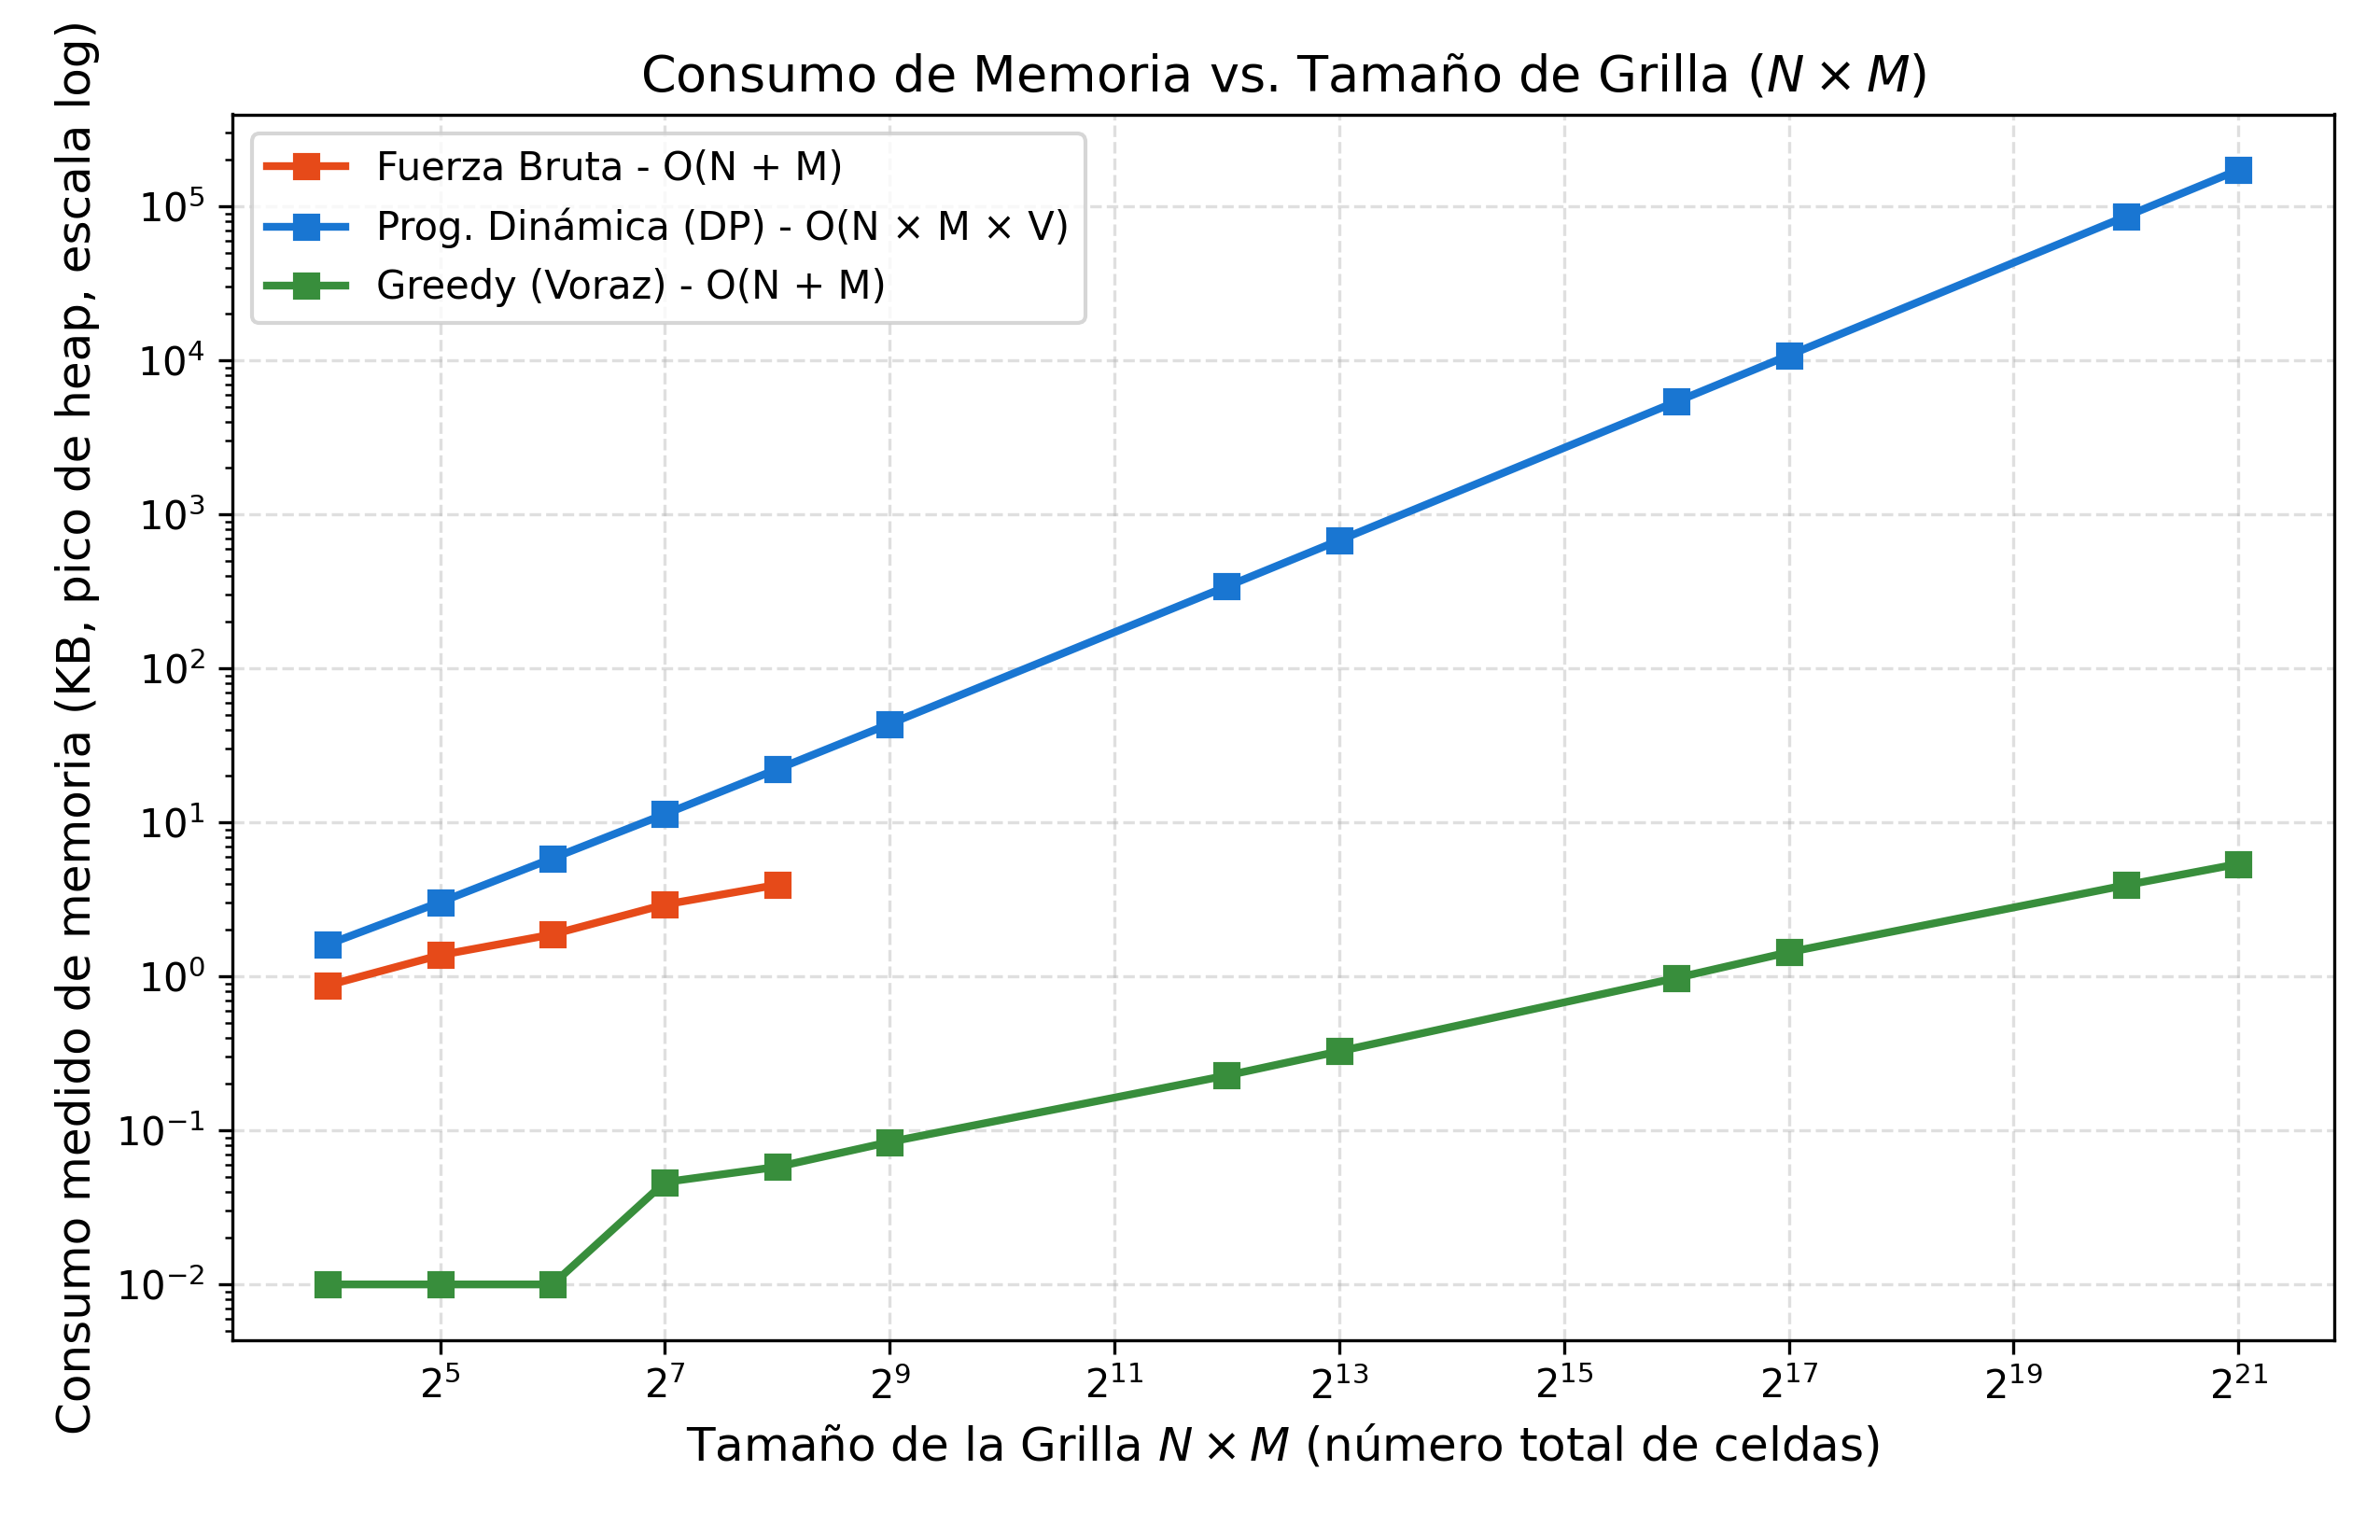
\includegraphics[width=0.83\linewidth]{../code/grid_pathfinding/data/plots/02_memoria_vs_tamano.png}
\caption{Consumo de memoria medido para cada algoritmo según el tamaño de la grilla.}
\label{fig:memoria}
\end{figure}




\subsection{Calidad de solución y tasa de falla de Greedy}

En todas las instancias pequeñas donde se ejecutaron ambos algoritmos 
exactos ($N+M \le 32$), la fuerza bruta y programación dinámica obtuvieron
los mismos puntajes, dando validez a programación dinámica como referencia óptima 
para evaluar el desempeño en todo el rango experimental.


\begin{table}[H]
\centering
\small
\caption{Tasa de falla de greedy por tipo de grilla y dominio ($36$ instancias por celda).}
\label{tab:falla}
\begin{tabular}{lrr}
\hline
Tipo de grilla & D10 & D1000 \\
\hline
Libre    & 0,0\%  & 0,0\% \\
Minas    & 0,0\%  & 2,8\% \\
Mixta    & 33,3\% & 13,9\% \\
Murallas & 22,2\% & 33,3\% \\
\hline
\end{tabular}
\end{table}

Como se observa en la Tabla~\ref{tab:falla} y en la Figura~\ref{fig:falla-tipo},
las fallas SIN SOLUCION se concentran en escenarios con 
obstáculos. En terrenos libres, greedy alcanza 
la meta en la totalidad de los casos, mientras que en grillas de 
murallas y mixtas la tasa de falla alcanza hasta un 
tercio de las instancias en murallas D1000 y mixtas D10,
producto de decisiones miopes que desvían hacia caminos
sin salida bloqueados por murallas o bordes del mapa. 
En terrenos de minas en el dominio D1000 se registra 
menores fallas, lo cual ocurre cuando reglas de desempate 
o celdas vecinas negativas inducen a agotar de 
forma temprana su margen de vidas ($V-1$) y quedar bloqueado al llegar 
con $v=1$ frente a nuevas minas. Por otro lado, 
la Figura~\ref{fig:falla-tamano} muestra que la evolución de la falla 
respecto al tamaño de la grilla varia en saltos discretos debido al 
número acotado de semillas aleatorias por dimensión, quedando en evidencia que 
el bloqueo de greedy depende de la configuración espacial 
específica de los obstáculos más que del tamaño del tablero.

\begin{figure}[H]
\centering
\subfloat[Tasa por tipo y dominio.\label{fig:falla-tipo}]{%
  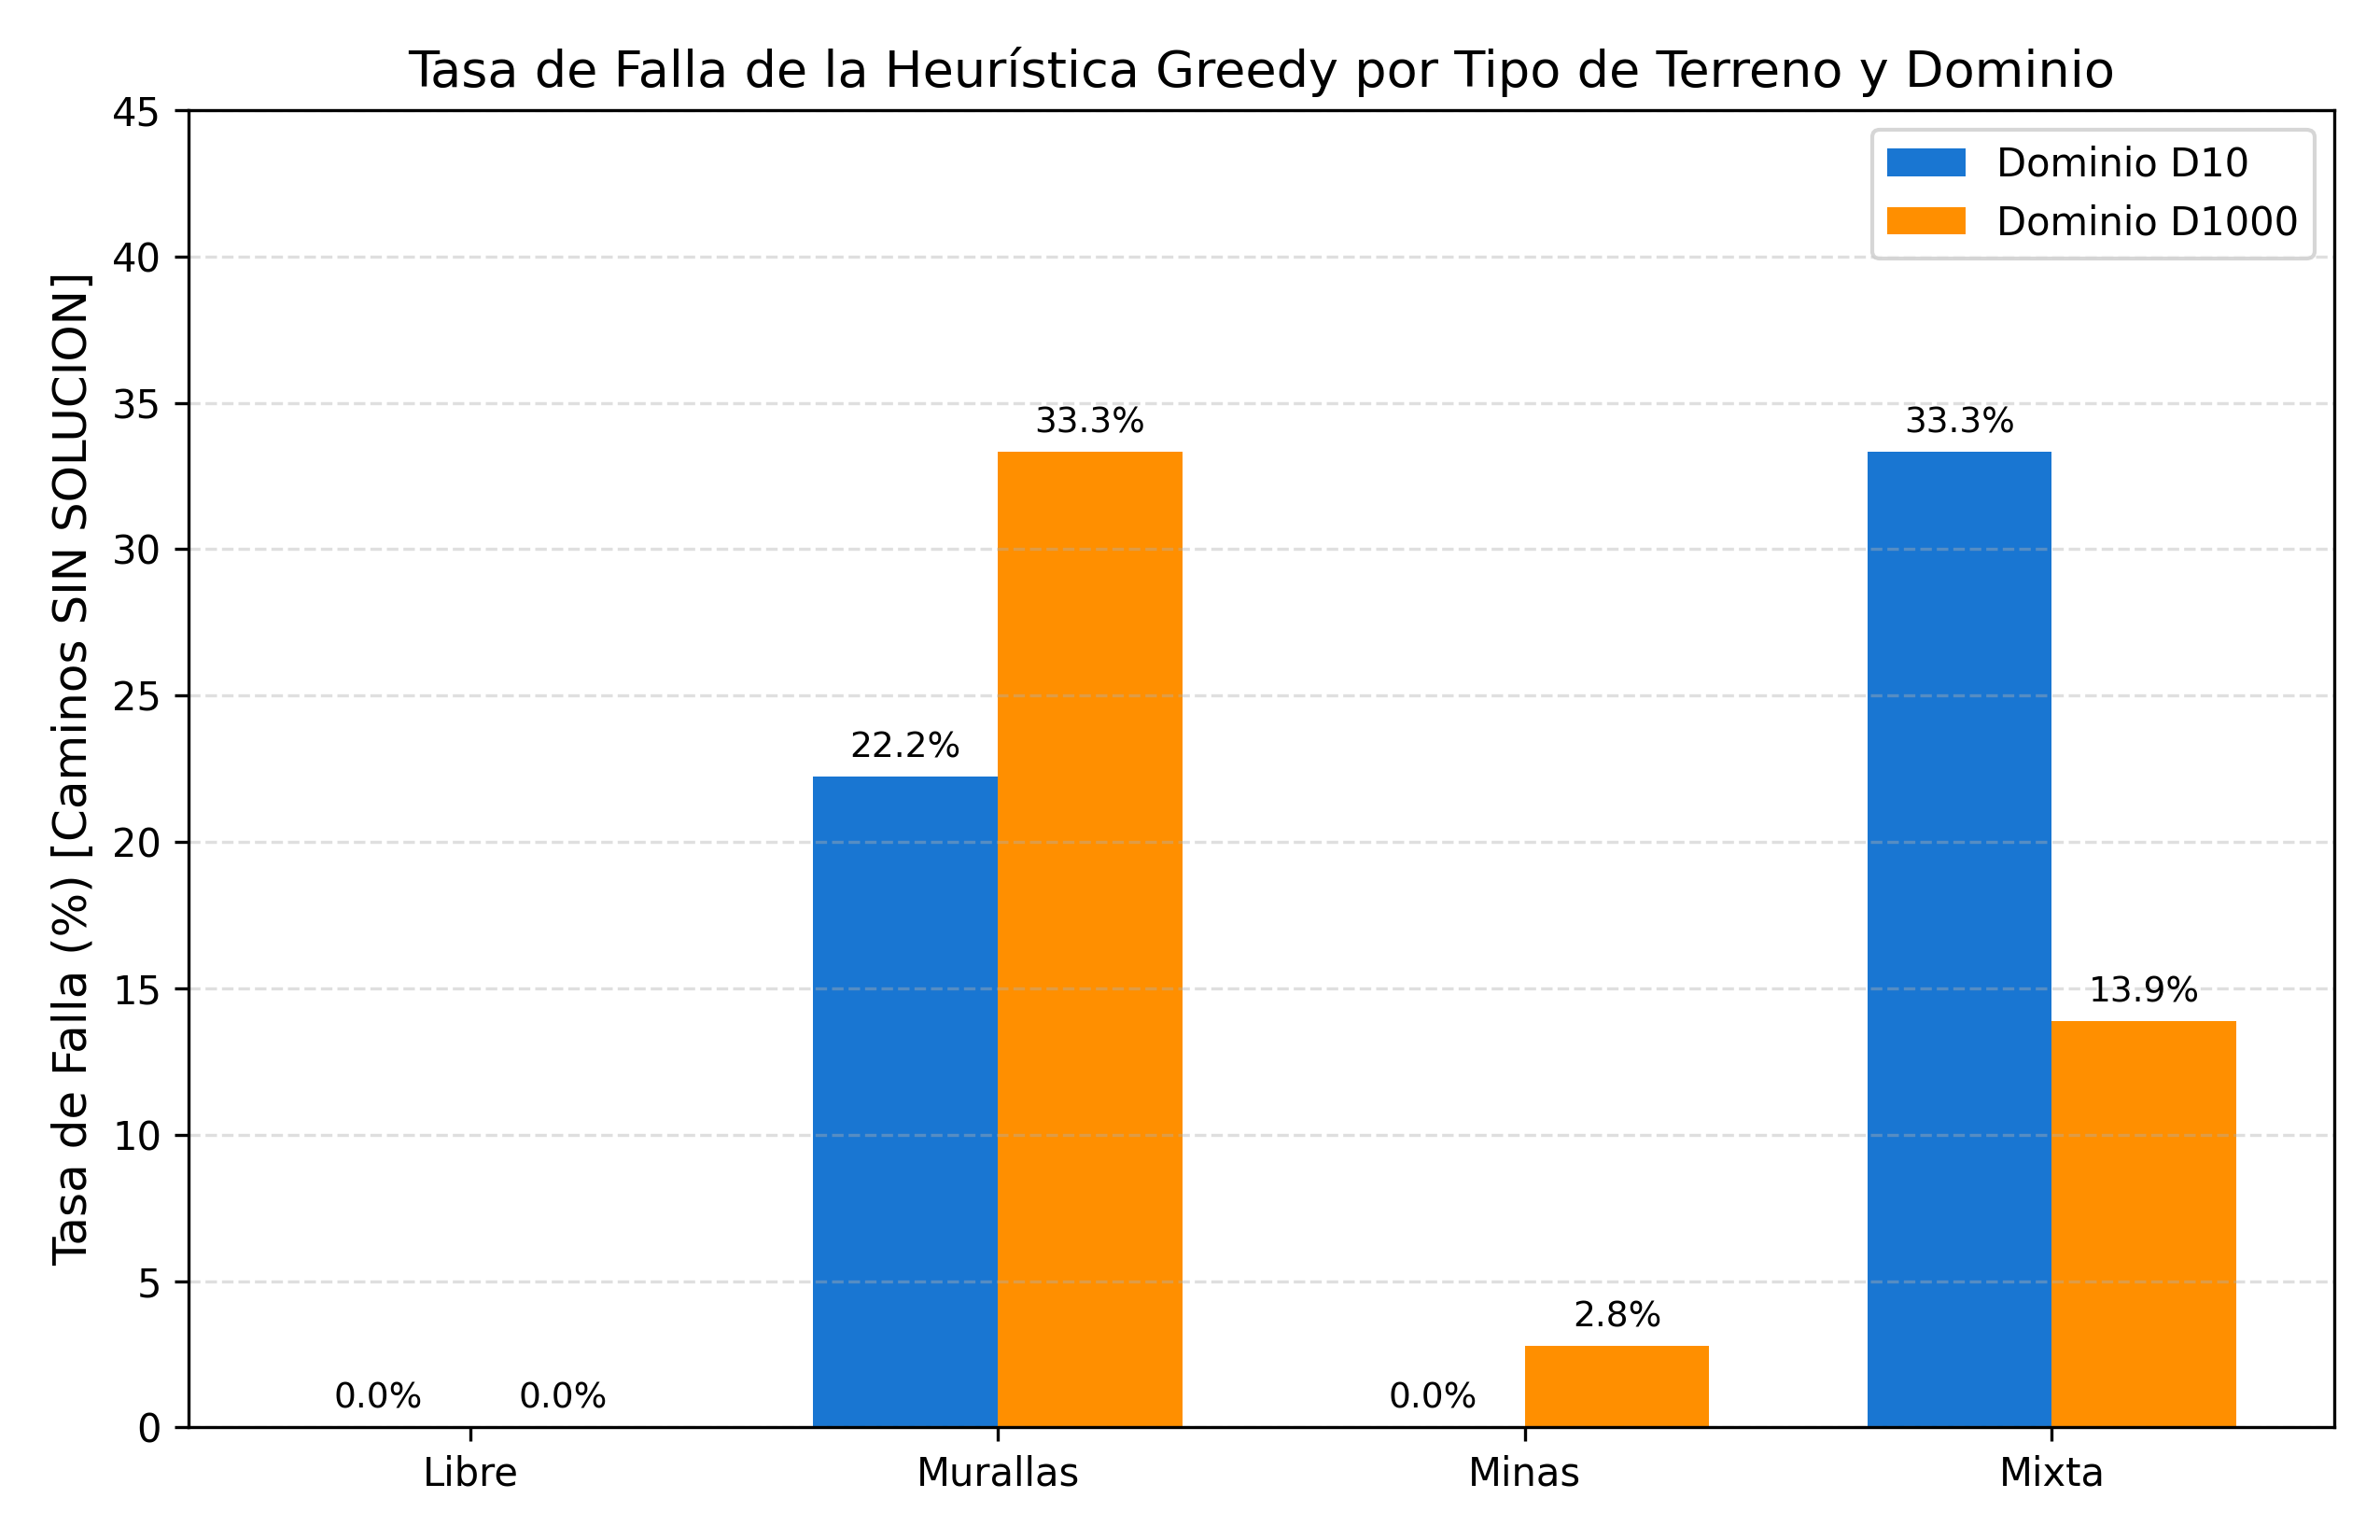
\includegraphics[width=0.48\linewidth]{../code/grid_pathfinding/data/plots/04_tasa_falla_greedy.png}}
\hfill
\subfloat[Tasa según tamaño en terrenos con obstáculos.\label{fig:falla-tamano}]{%
  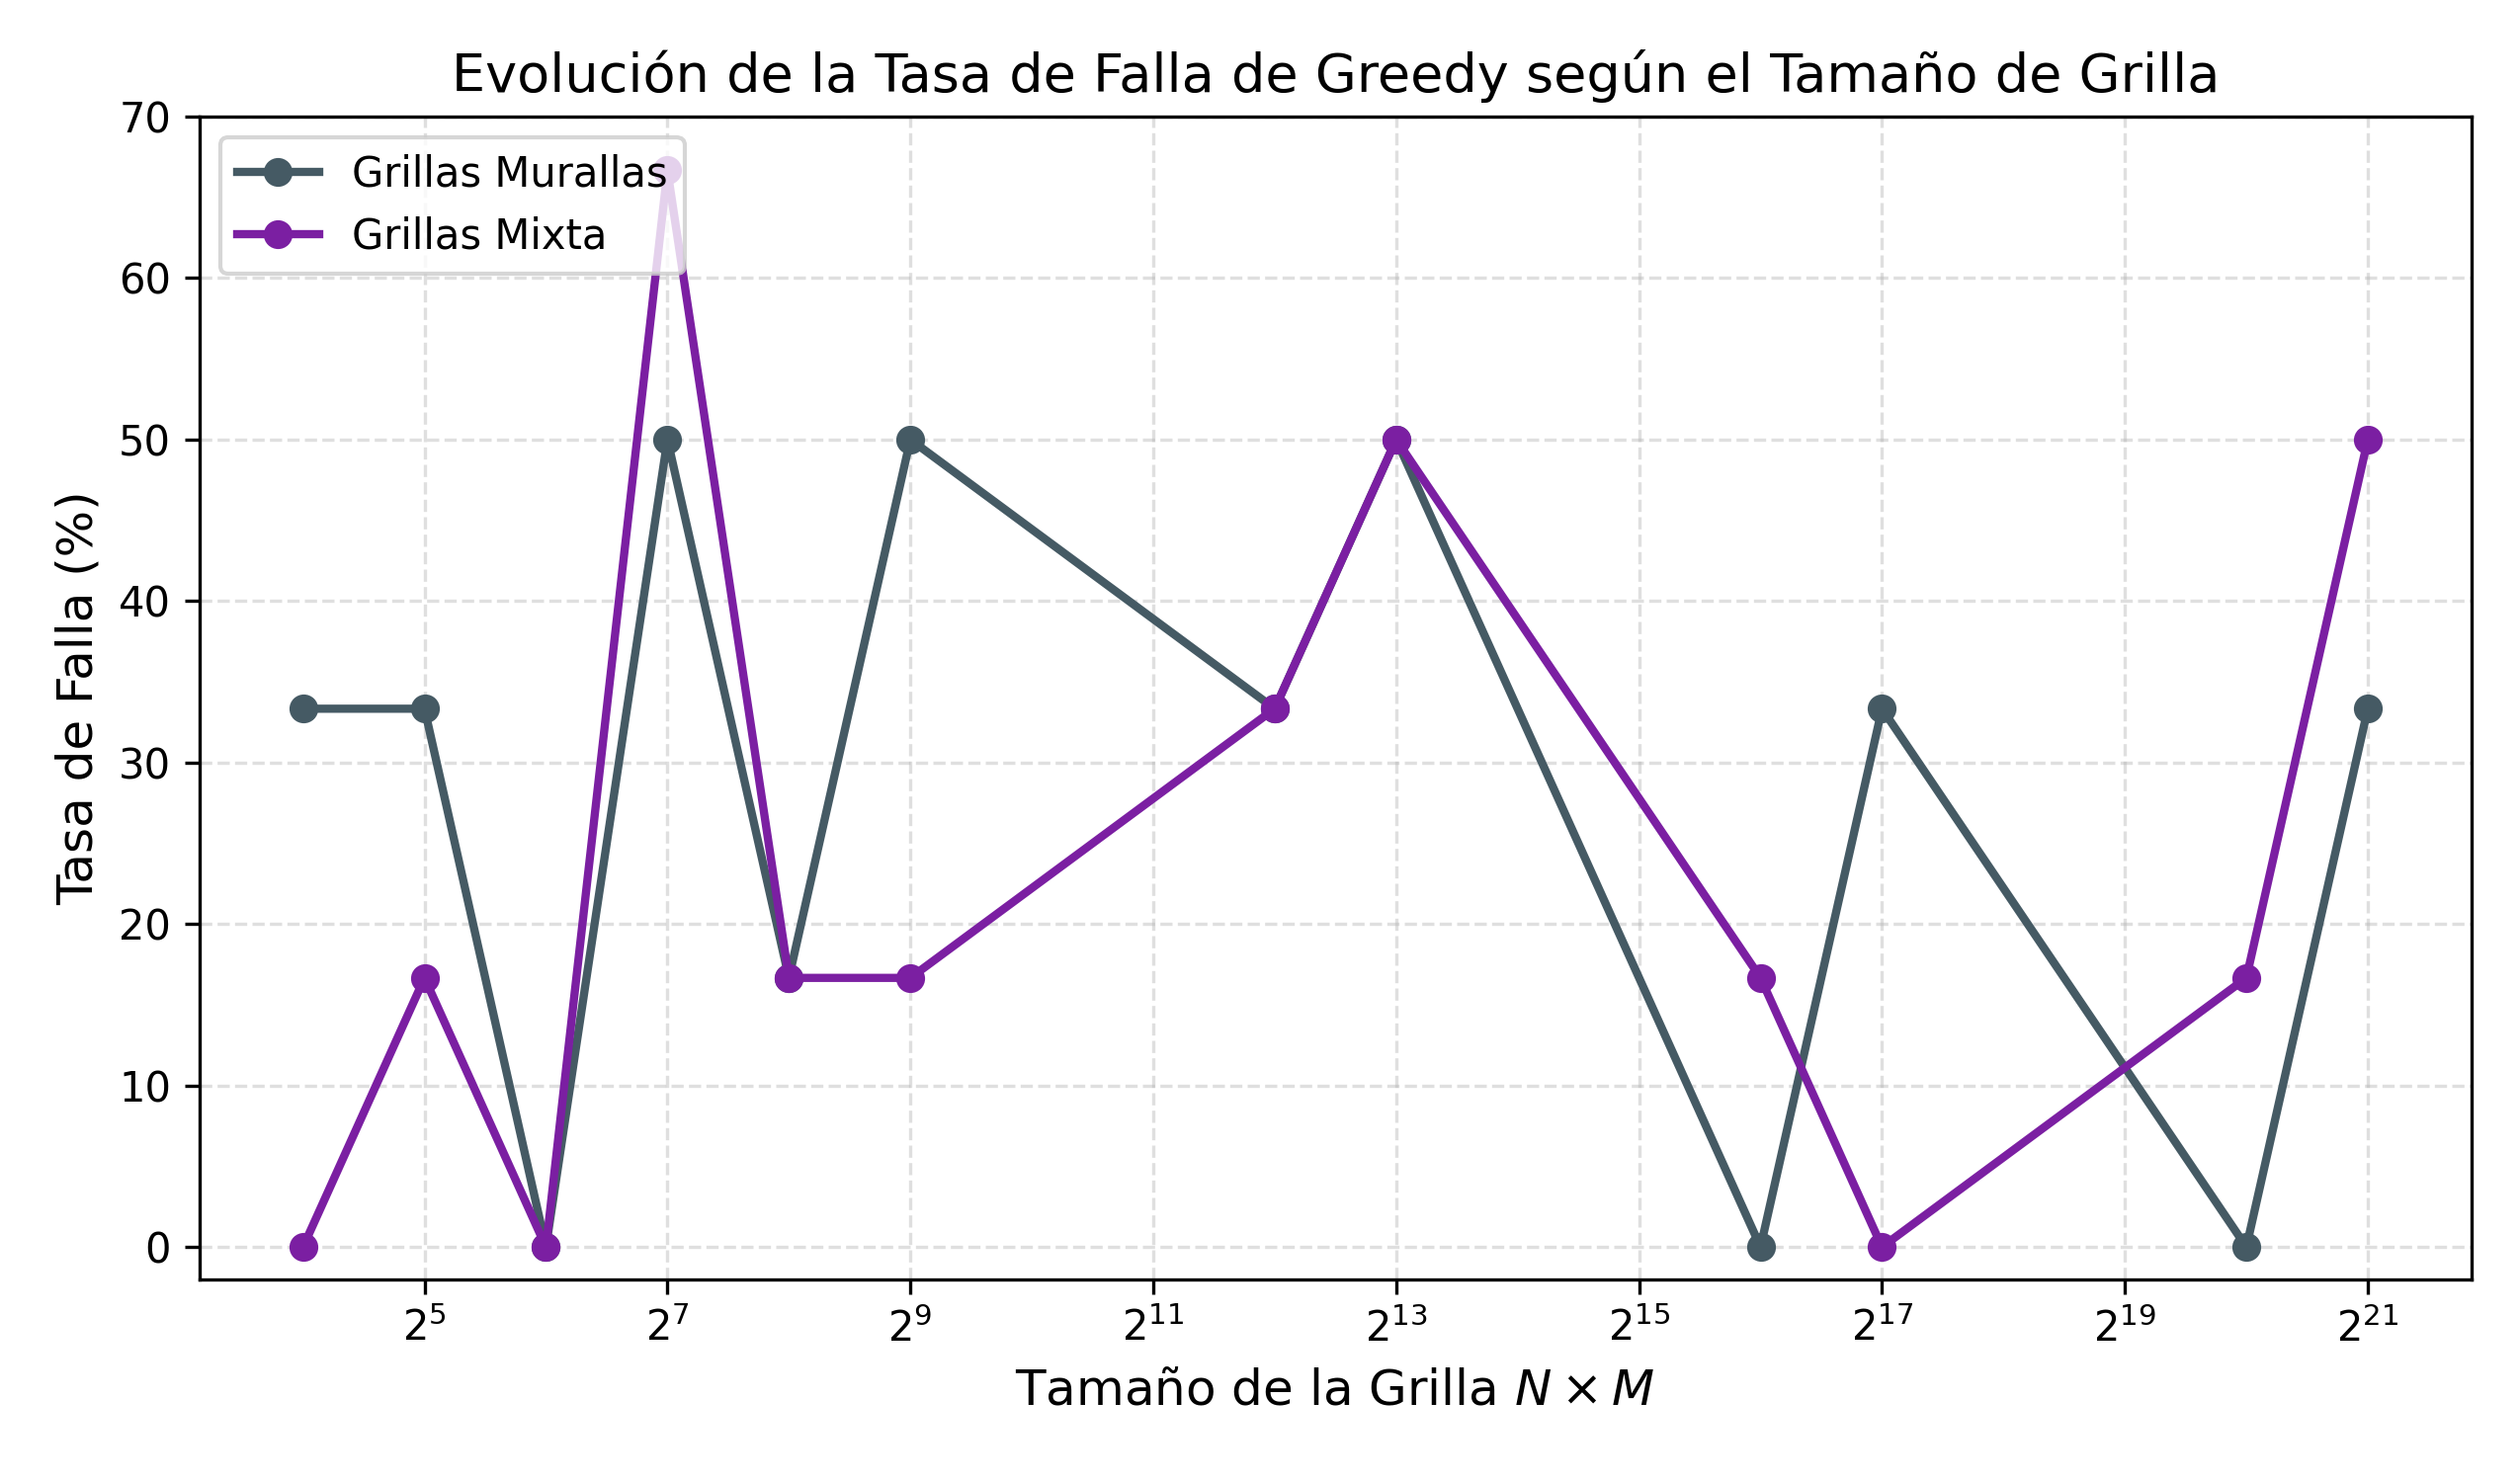
\includegraphics[width=0.48\linewidth]{../code/grid_pathfinding/data/plots/04b_tasa_falla_vs_tamano.png}}
\caption{Tasa de falla de greedy según terreno, dominio y tamaño.}
\label{fig:fallas}
\end{figure}

Para las instancias en que greedy logra alcanzar el destino, 
se analizó su brecha de optimalidad  $\Delta = s(C^*) \mathbin{\text{-}} s(C_{\text{greedy}})$,
excluyendo los casos fallidos para no distorsionar los promedios. En la Figura~\ref{fig:brecha} 
se aprecia que $\Delta$ 
presenta un crecimiento sostenido a medida que aumenta el tamaño 
de la grilla, reflejando la acumulación de decisiones locales subóptimas 
a lo largo de los $N+M-2$ pasos del recorrido. Al comparar ambos, 
la brecha en D1000 mantiene una escala dos ordenes de magnitud superior a 
la de D10, en correspondencia directa con el factor de escala entre los 
dominios de valores y las penalizaciones por mina,
esta diferencia de escala y la posibilidad de obtener puntajes óptimos 
nulos o negativos corroboran el uso de la brecha absoluta en lugar de una 
razón relativa, tambien en ambos dominios las curvas de los cuatro tipos de 
terreno se superponen, indicando que una vez que greedy 
logra completar un camino valido, la perdida acumulada respecto al óptimo 
está dirigido principalmente por la longitud del trayecto y la amplitud 
del dominio mas que por el tipo de obstáculo.

\begin{figure}[H]
\centering
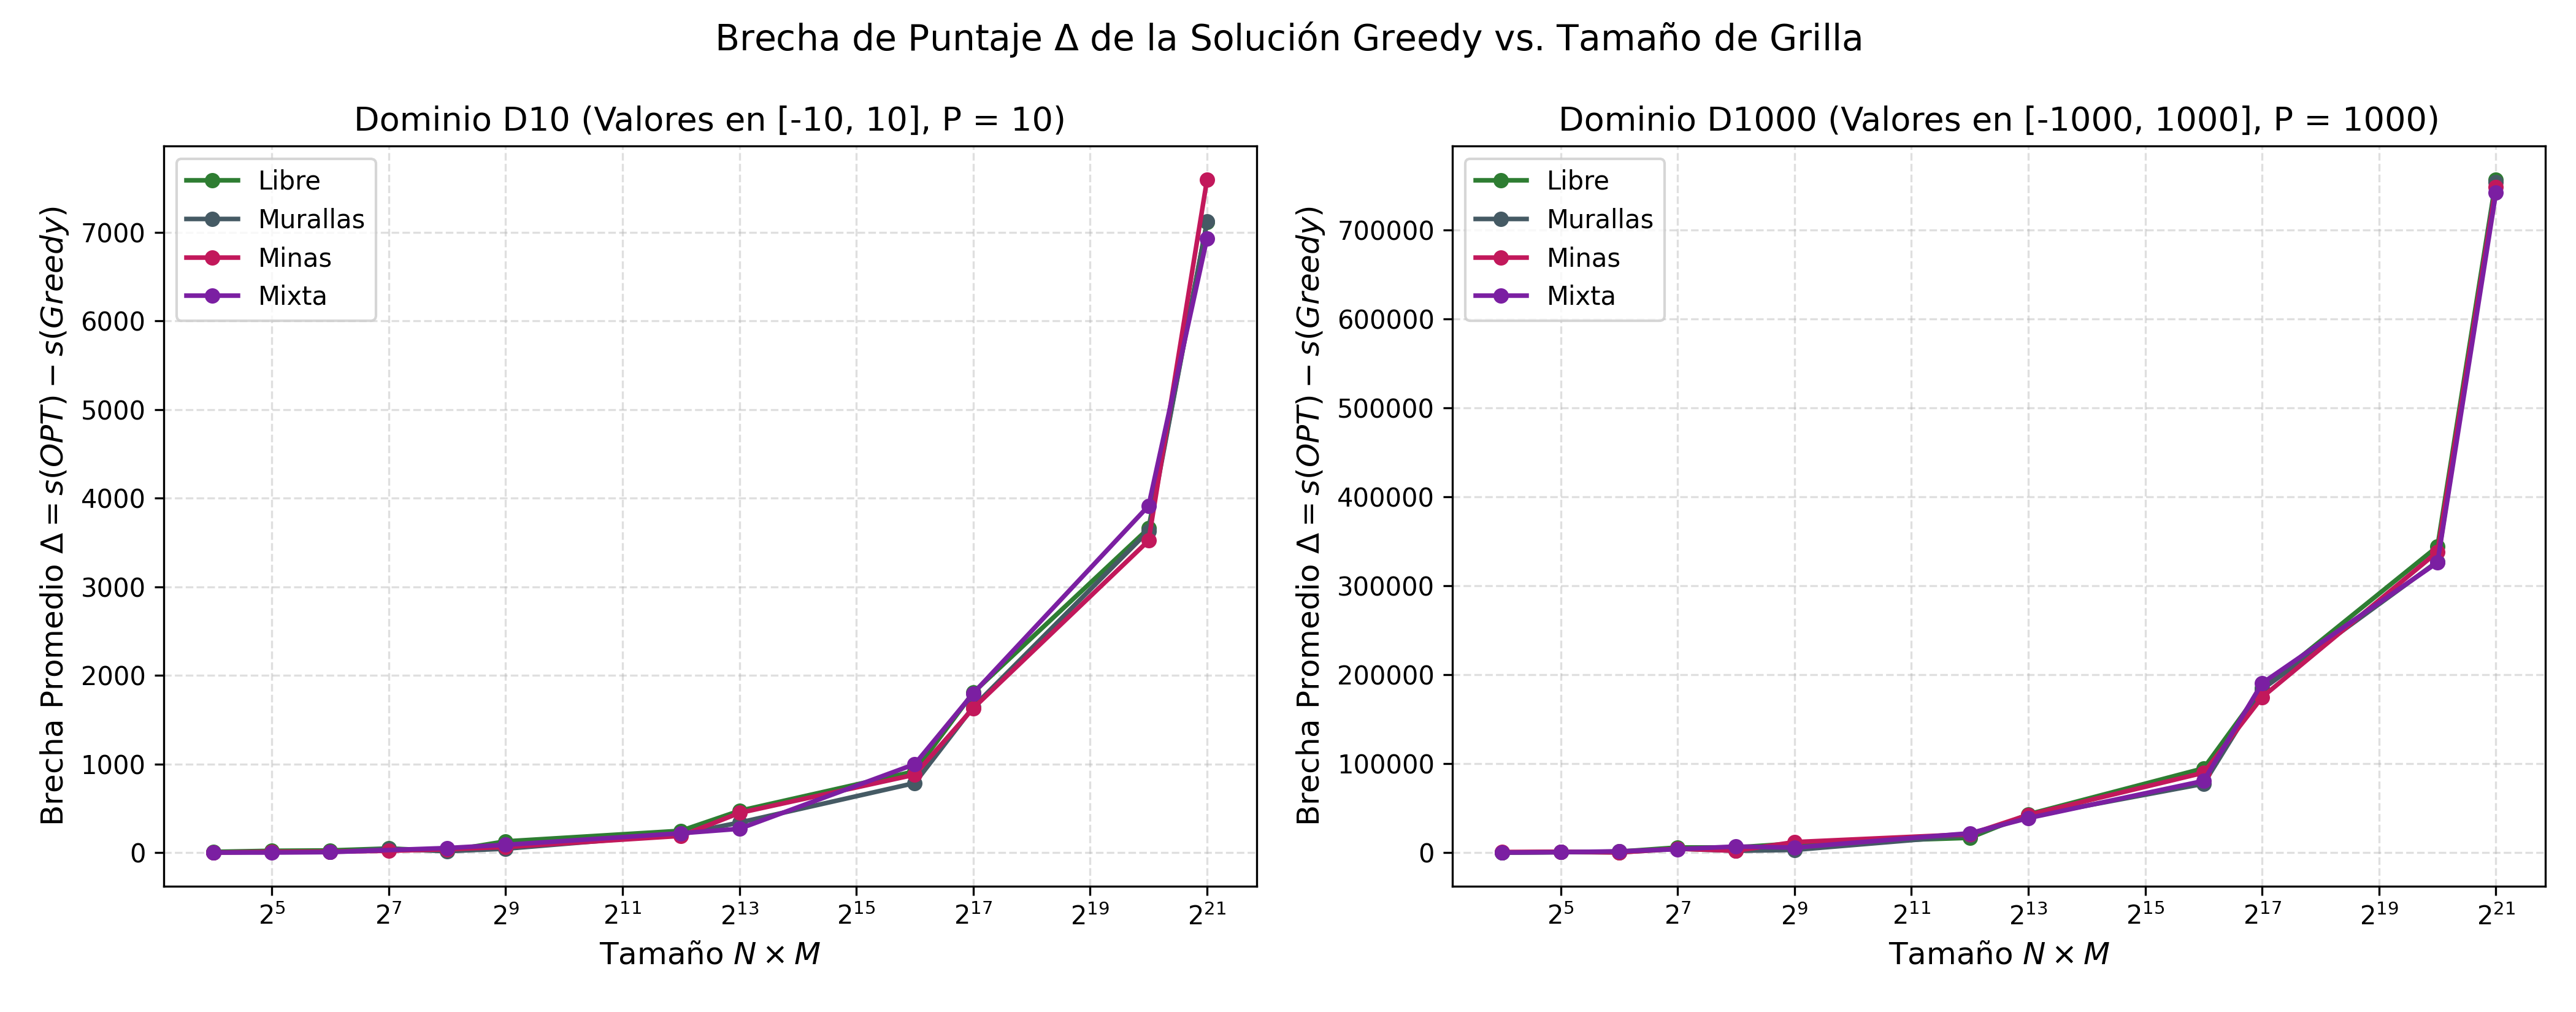
\includegraphics[width=0.83\linewidth]{../code/grid_pathfinding/data/plots/03_brecha_vs_tamano.png}
\caption{Brecha media de puntaje entre DP y greedy, considerando únicamente instancias donde greedy encuentra solución.}
\label{fig:brecha}
\end{figure}


\clearpage